%%%%%%%%%%%%%%%%%%%%%%%%%%%%%%%%%%%%%%%%%%%%%%
%%%%%%%%%%%%%%%%%%%%%%%%%%%%%%%%%%%%%%%%%%%%%%
%%			     Capitulo 1 			    %%
%%%%%%%%%%%%%%%%%%%%%%%%%%%%%%%%%%%%%%%%%%%%%%
%%%%%%%%%%%%%%%%%%%%%%%%%%%%%%%%%%%%%%%%%%%%%%

\chapter{Introducción} \label{cap1}
\setcounter{page}{1}
\pagenumbering{arabic}


\newpage

%%%%%%%%%%%%%%%%%%%%%%%%%%%%%%%%%%%%%%%%%%%%%%%%%%%%%%%
%			Seccion          					  %
%%%%%%%%%%%%%%%%%%%%%%%%%%%%%%%%%%%%%%%%%%%%%%%%%%%%%%%

\section{Motivación} \label{s1_1}
	
	\blindtext
	%\Blindtext
	
	
	\begin{figure}[htb]
		\centering
		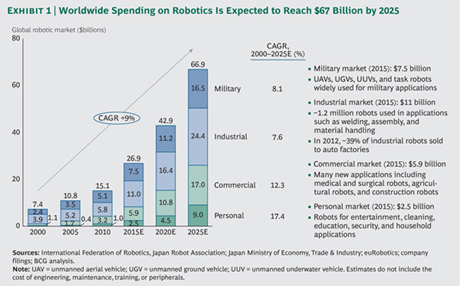
\includegraphics[width=0.6\linewidth]{capitulo_01/figuras_dir/crecimiento_robotica.png}
		\caption{Crecimiento previsto de la robótica entre los años 2000 y 2025}
		\label{Figura1_01}
	\end{figure} 
	
	Para citar un figura se puede realizar así: en la Fig. \ref{Figura1_01} puede verse el crecimientos estimado de la robótica.
	
	


\section{Objetivos} \label{s1_1_2}


	\blindtext
	
	Para poner un pie de página de  EDO\footnote{Ecuación diferencial ordinaria}
%%%%%%%%%%%%%%%%%%%%%%%%%%%%%%%%%%%%%%%%%%%%%%%%%%%%%%%
%			Seccion          					  %
%%%%%%%%%%%%%%%%%%%%%%%%%%%%%%%%%%%%%%%%%%%%%%%%%%%%%%%
\section{Alcance} \label{s1_2}

	\blindtext
	
	Para realizar un cita \citep{o2009wave}
%%%%%%%%%%%%%%%%%%%%%%%%%%%%%%%%%%%%%%%%%%%%%%%%%%%%%%%
%			Seccion				                      %
%%%%%%%%%%%%%%%%%%%%%%%%%%%%%%%%%%%%%%%%%%%%%%%%%%%%%%%
\section{Estructura de la memoria} \label{s1_3}
 
	\blindtext
	
	Esto es un ejemplo de una enumeración:
	\blindenumerate[3]
	
	Esto es un ejemplo de una lista: 
	\blinditemize[3]